\documentclass[12pt]{article}

\usepackage{fontawesome}
\usepackage{hyperref}
\usepackage{xurl}
\usepackage{graphicx}
\usepackage{float}
\usepackage[tagged, highstructure]{accessibility}
\usepackage{bookmark}
\usepackage{enumitem}

\hypersetup{
    colorlinks=false,
    pdfborder={0 0 0},
    pdftitle={NoSQL Scaling},
    pdfauthor={Adrianna Holden-Gouveia},
    pdfsubject={Advanced Data - Lab Assignment},
    pdflang={en-US},
    pdfkeywords={NoSQL, MongoDB, scalability, real-time analytics}
}

% Configure PDF bookmarks for navigation
\bookmarksetup{
    numbered,
    open,
}

% Configure list spacing for better accessibility
\setlist{nosep}



\title{NoSQL Scaling}
\author{
        Adrianna Holden-Gouveia \\
        Website: \href{https://aholdengouveia.name}{aholdengouveia.name}\\ 
        \date{\vspace{-5ex}}
        %Email: \href{mailto:admin@aholdengouveia.name}{admin@aholdengouveia.name} \\
%        \faLinkedin{: aholdengouveia} \\
        \faGithub {: aholdengouveia} \\
        %\faTwitter {: aholdengouveia} \\
        }

%S\date{\today}


\begin{document}    

\maketitle

%\begin{abstract}
%This is a template for Linux Administration Lab work
%\end{abstract}
%\tableofcontents


\section*{Accessibility Notice}
This document is also available in HTML format at:

Link: \href{https://aholdengouveia.name/AdvData/labs/wk12nosqlscaling.html}{\textbf{\nolinkurl{https://aholdengouveia.name/AdvData/labs/wk12nosqlscaling.html}}}

The HTML version provides enhanced accessibility features including keyboard navigation, screen reader support, responsive design, dark mode support, and high contrast options.

\section*{Request}
\noindent\textbf{Request:} DATA-5317\\
\textbf{Requested by:} Head of the data team\\
\textbf{Data:} Your database, and your data collection plan from the Big Data lab

\section*{Background}
Some of the new data in your collection plan doesn't fit neatly into tables. Before the company commits to anything, your manager wants you to try a NoSQL document database with your own data, decide what the company should give up if its database servers ever lose contact with each other, and recommend how a NoSQL database should be hosted.

\section*{Learning Outcomes}
By the end of this lab, you will be able to:
\begin{itemize}
    \item Store and query data in a NoSQL document database
    \item Compare document and relational models for a data set
    \item Explain the trade-offs of the CAP theorem for a business
    \item Recommend a way to host a NoSQL database, including cost and vendor lock-in
\end{itemize}

\section*{Lab Instructions}
Use your own data set and company. Books are my example data only.

\subsection*{Screenshots}
Several parts of this lab ask for a screenshot. Each screenshot should have your name, term, and year.  One of the easiest ways to do that is make a text document with your name and term/year on your computer and save it to use all term. Any screenshots that don't include this information won't be counted.

\begin{figure}[H]
    \centerline{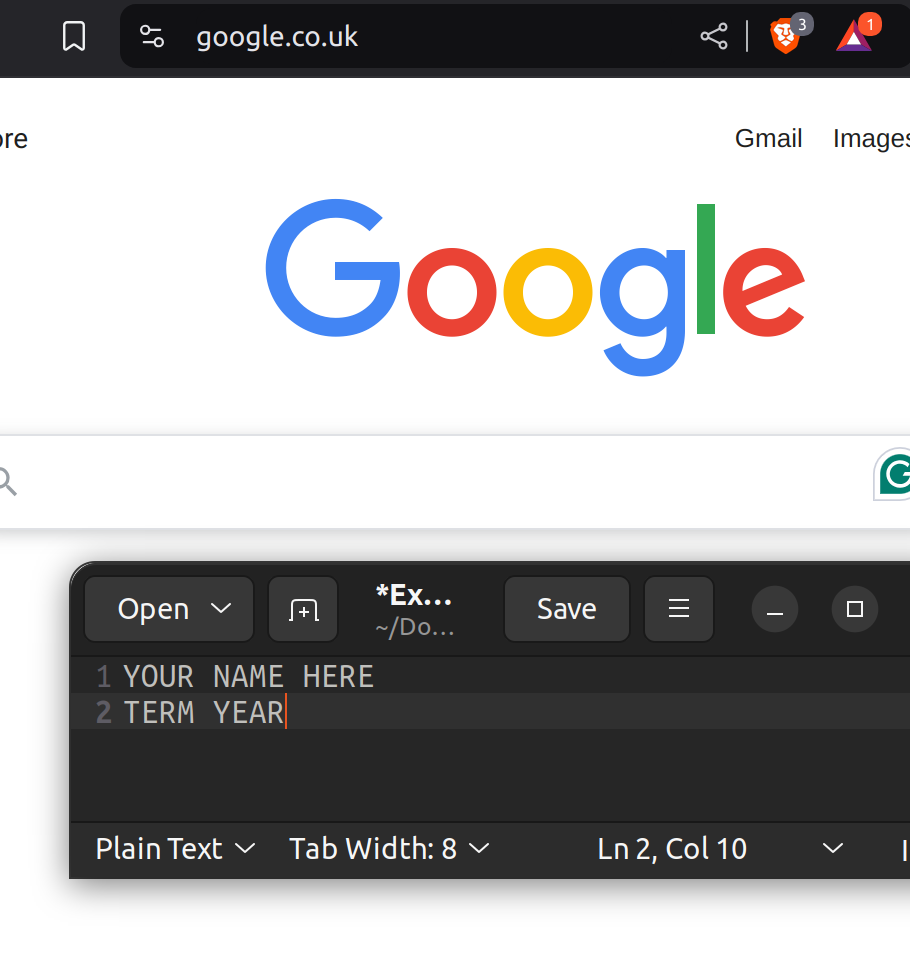
\includegraphics[scale=.2]{ExampleScreenshot.png}}
    \caption{This is an image of what each of your screenshots should look like}
    \alt{Example screenshot: a web browser showing the Google home page, with a small text editor window in front of it that says YOUR NAME HERE and TERM YEAR}
\end{figure}

\subsection*{Part 1: NoSQL Training}
Pick a free course at MongoDB University (linked under Resources). You'll need a free account. Don't pay for anything; if a course isn't free, talk to me. If you're not sure what to pick, try Introduction to MongoDB. You don't have to finish it, but go through at least the section MongoDB CRUD Operations: Replace and Delete Documents.
\begin{enumerate}
    \item Take a screenshot of your progress in the course.
    \item Which course did you pick, and how much of it did you do?
    \item What did you think of it? Was it hard, easy, or time consuming?
    \item Which concepts did you try out, and what would you want to learn next?
\end{enumerate}
\textbf{Optional, not required for this class:} if you finish a course, you can earn a certificate of completion to put on your resume.

\subsection*{Part 2: Fit Check}
Any data can be stored in a document database, but some data fits better than others. Check your main data set for these 4 signs, and give an example from your data for each one you find:
\begin{enumerate}
    \item Lists stored in one cell, like several genres in one column
    \item Fields that only some rows have, like a series name that most books don't have
    \item Information that naturally nests inside something else, like an author's details inside a book
    \item Records that vary in shape, where different rows need different columns
\end{enumerate}
If your main data shows at least one of these signs, use it in Part 3. If it shows none, that's a real finding: your data fits tables well. You'll still use it in Part 3, and you'll also add new data from your data collection plan that doesn't fit neatly into tables, such as reviews or website activity.

\subsection*{Part 3: Documents in Mongo Playground}
Mongo Playground (linked under Resources) runs MongoDB in your browser, with nothing to install and no account. Follow the sample NoSQL documents (linked under Resources). Copy from the sample text file, not from this PDF, since quote marks from a PDF often cause errors.
\begin{enumerate}
    \item In the Database box, write 3 to 5 documents from your own data. Nest related information inside a document, and use a list for anything with more than one value.
    \item Add at least 1 document of new data from your data collection plan, with different fields from the others.
    \item Run at least 2 find queries, including one that filters, such as finding documents with a certain value. Take a screenshot of each query and its results.
    \item Compare your documents to your tables from the Beyond SQL lab. What is easier with documents? What is harder? For example, if information is copied into many documents, what happens when it changes?
\end{enumerate}

\subsection*{Part 4: The CAP Theorem}
When a database is spread across servers, the network between them will sometimes fail. The CAP theorem says that when it does, the database has to choose between consistency, where every answer is up to date or there's an error, and availability, where every request gets an answer even if it might be out of date.
\begin{enumerate}
    \item Explain consistency, availability, and partition tolerance in your own words.
    \item Pick 2 kinds of data at your company: one where consistency matters more, and one where availability matters more. For example, a store's stock count must be right, but a review that shows up a few minutes late doesn't hurt anyone. Explain each choice.
    \item If your company could only pick one for its whole database, which should it be, and why?
\end{enumerate}

\subsection*{Part 5: Hosting Recommendation}
The topic page describes 3 ways to run a NoSQL database: a third party that runs it for you (Database-as-a-Service), a virtual machine hosted by a cloud company that your own staff run, and a middle ground where the cloud company hosts the database for you. Research the options, using at least 2 reliable sources checked with the CRAAP test (linked under Resources), and cite each one with a link.

Write a memo of about one page to the finance director recommending one option, following the sample recommendation memo from the Database Matchmaking lab (linked under Resources). Base it on your company's size and staff skills, and include the cost, including any hidden costs such as consultants, and the risk of vendor lock-in, where it's hard to switch away later.

\textbf{Optional, not required for this class:} give 3 examples of real-time analytics your company could do with the new data in your data collection plan. Be specific.

\section*{Acceptance Criteria}
This request is done when:
\begin{itemize}
    \item Your MongoDB course has a screenshot and answers to all 4 questions
    \item Your fit check covers all 4 signs, with examples from your own data
    \item At least 3 documents from your own data and 1 of new data, using nesting and a list
    \item At least 2 find queries, one with a filter, each with a screenshot of the results
    \item Your comparison names at least one thing that's easier and one that's harder with documents
    \item Your CAP answers use 2 real kinds of data from your company
    \item Your hosting memo leads with a recommendation, covers cost and vendor lock-in, and cites at least 2 sources you've checked with the CRAAP test
    \item Every screenshot follows the screenshot rules
\end{itemize}

\section*{Deliverables}
One file that includes Parts 1 to 5, and the optional real-time analytics examples if you do them.

Audience: the head of the data team for Parts 1 to 4. The memo in Part 5 is for the finance director, who isn't technical.

\section*{Resources}
References, a video, a PowerPoint and some notes are available at my website
Link: \href{https://www.aholdengouveia.name/AdvData/NoSQLscaling.html}{\textbf{\nolinkurl{https://www.aholdengouveia.name/AdvData/NoSQLscaling.html}}}

MongoDB University free courses
Link: \href{https://learn.mongodb.com/}{\textbf{\nolinkurl{https://learn.mongodb.com/}}}

Mongo Playground, runs MongoDB in your browser
Link: \href{https://mongoplayground.net/}{\textbf{\nolinkurl{https://mongoplayground.net/}}}

Sample NoSQL documents and queries, for Part 3
Link: \href{https://www.aholdengouveia.name/AdvData/labs/SampleNoSQLDocuments.txt}{\textbf{\nolinkurl{https://www.aholdengouveia.name/AdvData/labs/SampleNoSQLDocuments.txt}}}

Sample recommendation memo, for Part 5
Link: \href{https://www.aholdengouveia.name/AdvData/labs/SampleRecommendationMemo.txt}{\textbf{\nolinkurl{https://www.aholdengouveia.name/AdvData/labs/SampleRecommendationMemo.txt}}}

The CRAAP test, for checking your sources
Link: \href{https://web.archive.org/web/20250814000638/https://guides.lib.uchicago.edu/c.php?g=1241077&p=9082343}{\textbf{\nolinkurl{https://web.archive.org/web/20250814000638/https://guides.lib.uchicago.edu/c.php?g=1241077&p=9082343}}}

My guide to evaluating sources
Link: \href{https://www.aholdengouveia.name/Howtos/Sourceeval/sourceEvaluation.html}{\textbf{\nolinkurl{https://www.aholdengouveia.name/Howtos/Sourceeval/sourceEvaluation.html}}}

\end{document}